\documentclass[10pt,a4paper]{report}
\usepackage[utf8]{inputenc}
\usepackage[spanish]{babel}
\usepackage{amsmath}
\usepackage{amsfonts}
\usepackage{amssymb}
\usepackage{makeidx}
\usepackage{graphicx}
\usepackage{titlesec}
\usepackage{sectsty}
\usepackage{listings}
\usepackage{color}
\usepackage{float}
\usepackage{hyperref}
\usepackage{apacite}

\titleformat{\chapter}[display]
{\normalfont\bfseries}{}{0pt}{\Large}
\chaptertitlefont{\Huge}

\definecolor{codegreen}{rgb}{0,0.6,0}
\definecolor{codegray}{rgb}{0.5,0.5,0.5}
\definecolor{codepurple}{rgb}{0.58,0,0.82}
\definecolor{backcolour}{rgb}{0.95,0.95,0.92}

\lstdefinestyle{mystyle}{
	backgroundcolor=\color{backcolour},   
	commentstyle=\color{codegreen},
	keywordstyle=\color{magenta},
	numberstyle=\tiny\color{codegray},
	stringstyle=\color{codepurple},
	basicstyle=\footnotesize,
	breakatwhitespace=false,         
	breaklines=true,                 
	captionpos=b,                    
	keepspaces=true,                 
	numbers=left,                    
	numbersep=5pt,                  
	showspaces=false,                
	showstringspaces=false,
	showtabs=false,                  
	tabsize=2,
	frame=lines
}

\lstset{style=mystyle}

\author{Medina Medina, David A.\\}
\title{Práctica 10 - Jugando al \textit{Pong} con un sensor de distancia}
\begin{document}
	\maketitle
	\tableofcontents
	\bibliographystyle{apacite}
	\chapter{Introducción}
	\textit{Arduino} es el primer proyecto de hardware en open-source que facilita el diseño de productos digitales que requieren de un microcontrolador.
	
	El objetivo de este proyecto \cite{repositorio-github} consiste en utilizar la placa \textit{Arduino UNO R3} para leer los datos que nos llegan del sensor de distancia \textit{GP2D12}. Este sensor será utilizado para mover el jugador derecho del juego \textit{Pong} que se implementó en la práctica 1.
	
	Este documento describe los cambios más importantes que se han realizado en el diseño del proyecto de la práctica 1 además del código que se ha diseñado para que la placa \textit{Arduino Uno R3} lea y transmita la información del sensor de proximidad a \textit{Processing}.
	
	
	\chapter{Método y materiales}
	\section{Materiales}
	El desarrollo de este proyecto se ha llevado a cabo utilizando el IDE de desarrollo de aplicaciones \textit{C/C++} y \textit{Java} de \textit{JetBrains}, \textit{CLion} e \textit{IntelliJ}, respectivamente. El resto de materiales hardware/software utilizados en este proyecto son enumerados a continuación:
	\begin{itemize}
		\item Placa Arduino Uno R3.
		\item Sensor de distancia \textit{GP2D12}.
		\item Librería \texttt{Arduino.h} \cite{arduino-reference}.
		\item Archivo \texttt{CMakeLists.txt} para la construcción automatizada de las dependencias de la librería \texttt{Arduino.h}.
		\item Librería \texttt{Serial} de \textit{Processing}.
	\end{itemize}

	El proyecto también puede cargarse en la placa usando el el IDE oficial de \textit{Arduino}.  
	
	\section{Método}
	El desarrollo de este proyecto se divide en dos categorías importantes:
	\begin{itemize}
		\item Lectura de medidas del sensor de proximidad.
		\item Adapatación del código del \textit{Pong}.
	\end{itemize}
	
	\subsection{Lectura de medidas del sensor de proximidad}
	El código que se cargará en la placa \textit{Arduino Uno R3} se encuentra el el archivo \texttt{Practica10.ino} el cual se estructura en las siguientes partes:
	\begin{itemize}
		\item Rutina \texttt{setup()}.
		\item Rutina \texttt{loop()}.
		\item Rutina \texttt{signalScaling()}
	\end{itemize}

	\subsubsection{Rutina \texttt{setup()}}\label{subsub:setup}
	Esta primitiva realiza los ajustes iniciales de la placa. Se establece la velocidad de transmisión de datos de la placa a 115200 baudios. 
	
	El fabricante indica el tiempo de duración de la primera medida con datos espúrios que obtenemos del sensor (ver figura \ref{fig:gp2d12-espera}). El tiempo de duración esta primera lectura es de $38.3 ms \pm 9.6ms$. El tiempo transcurrido entre el final de la primera lectura y el comienzo de la siguiente es como máximo de $5ms$.
	
	Por este motivo, se establece un tiempo de espera inicial con la primitiva \texttt{delay()} de $43ms$.
	
	\lstinputlisting[language=C++, firstline=5, lastline=8]{../src/Arduino-Sensor/Practica10.ino}
	
	\begin{figure}[H]\label{fig:gp2d12-espera}
		\centering
		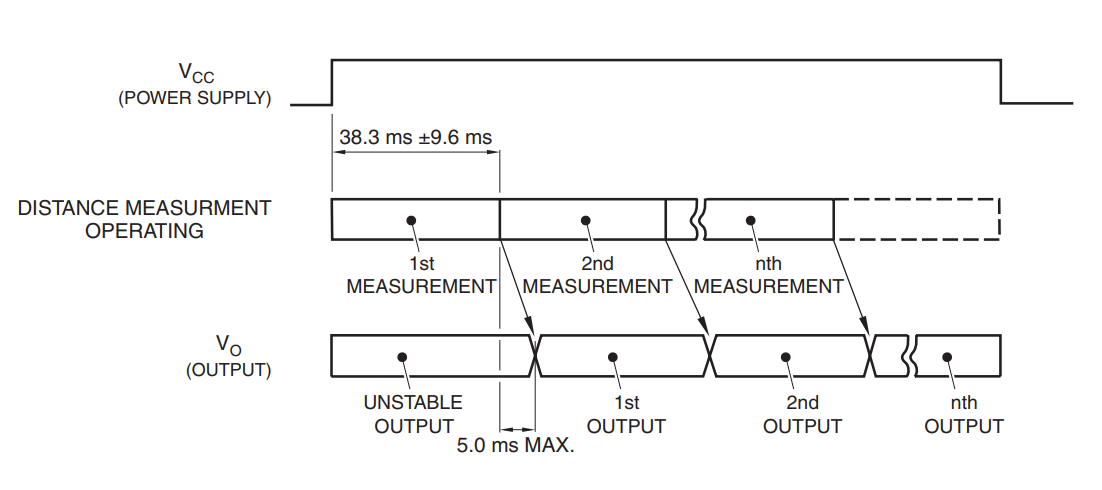
\includegraphics[width=0.75\textwidth]{time-diagram.png}
		\caption{Diagrama de tiempo del sensor \textit{GP2D12}}
	\end{figure}
	
	\subsubsection{Rutina \texttt{loop()}}
	Esta rutina primitiva define el bucle principal que se ejecuta en la placa \textit{Arduino}. 
	
	La variable \texttt{val} contiene el valor de las medidas leídas del sensor tras llamar a la rutina \texttt{signalScaling()}.
	
	Por último, se manda el valor de \texttt{val} al puerto serial llamando a la primitva \texttt{Serial.println()} y se establece un tiempo de espera de $100ms$ entre lecturas.
	
	\lstinputlisting[language=C++, firstline=10, lastline=14]{../src/Arduino-Sensor/Practica10.ino}
	
	\subsubsection{Rutina \texttt{signalScaling()}}
	En esta rutina se extraen las medidas tomadas del sensor de proximidad utilizando la primitiva \texttt{analogRead()} y el pin analógico \texttt{A0}. Según la documentación oficial de \textit{Arduino} \cite{resolucion-analogica}, la resolución máxima de lectura analógica es de 10 bits para voltajes máximos de $5V$. Esta resolución permite valores en el intervalo $[0, 1023]$.
	
	Según el fabricante, el valor voltaje máximo de salida es de $2.6V$ para una distancia de $10cm$ (ver figura \ref{fig:voltaje-max}). Esto requiere ajustar la salida que obtenemos con \texttt{analogRead()} para un voltaje máximo de $2.6$. Se ha obtado también por reducir la resolución máxima original de 10 bits a 1 byte (valores en el intervalo $[0, 255]$), coincidiendo así el tamaño con el utilizado en la codificación \textit{ASCII}.
	
	Se aplica la siguiente fórmula para realizar las transformaciones pertinentes,
	
	\begin{equation*}
		x^\prime = x \cdot \frac{1023}{2.6} \cdot \frac{5}{1023} \cdot \frac{255}{1023} \
	\end{equation*}
	
	siendo $x^\prime$ el nuevo valor de salida con los escalados pertinentes y $x$ la medida obtenida en crudo del sensor.
	
	\begin{figure}[H]\label{fig:voltaje-max}
		\centering
		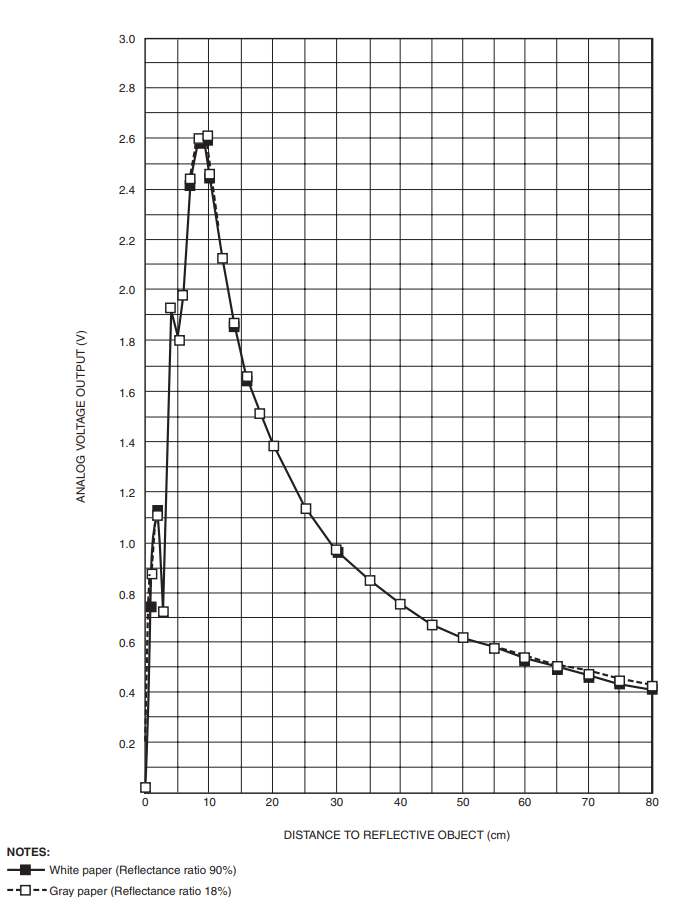
\includegraphics[width=0.75\textwidth]{volatje-max.png}
		\caption{Curva de distancia del sensor a la superficie reflectante frente al voltaje de salida}
	\end{figure}

	\lstinputlisting[language=C++, firstline=16, lastline=18]{../src/Arduino-Sensor/Practica10.ino}
	
	\subsection{Adapatación del código del \textit{Pong}}
	En este apartado se describe como se integra las medidas obtenidas del sensor de proximidad en \textit{Processing} haciendo uso de la librería \texttt{Serial}. Los pasos realizados se describen a continuación:
	
	\begin{enumerate}
		\item Modificación de la primitiva \texttt{setup()}.
		\item Generación de eventos en el puerto serie.
	\end{enumerate}
	
	\subsubsection{Modificación de la primitiva \texttt{setup()}}
	Justo al final de la primitiva \texttt{setup()}, se inicializa un puerto serie de lectura a 115200 baudios (ver \ref{subsub:setup}) creando un objeto \texttt{Serial}.
	
	Una vez establecida la comunicación serial, se inicializa un buffer a partir del cual se cargan las lecturas recibidas por el canal serial hasta alcanzar el caracter de salto de línea (\texttt{0x0A}), en cuyo caso se lanza un evento que llama a la rutina \texttt{serialEvent()}.
	
	\lstinputlisting[language=Java, firstline=58, lastline=73]{../src/Processing-Pong/src/Pong.java}
	
	En esta rutina, se lee la \textit{string} obtenida por el puerto serie y siempre y cuando lo que se reciba sea un número, se ajusta el valor de la componente vertical de la raqueta de la izquierda a un valor entre 0 y el alto máximo de la ventana. Este mapeo entre el dato obtenido por el puerto serie y la coordenada Y que le corresponde a la raqueta de la izquierda se consigue llamando a la primitiva \texttt{map()} de \textit{Processing}.
	
	\lstinputlisting[language=Java, firstline=147, lastline=153]{../src/Processing-Pong/src/Pong.java}
	
	\chapter{Conclusiones}	
	Hemos observado cómo es posible establecer una comunicación entre la información obtenida de un sensor de proximidad y un computador utilizando la comunicación serial para ello.

	La integración de lectura del puerto serie con \textit{Processing} abre las puertas a un abanico enorme de posibilidades para utilizar cualquier sensor hardware para interaccionar directamente con el ordenador a partir de una interfaz gráfica que nosotros diseñemos.
	
	\begin{figure}[H]\label{fig:res1}
		\centering
		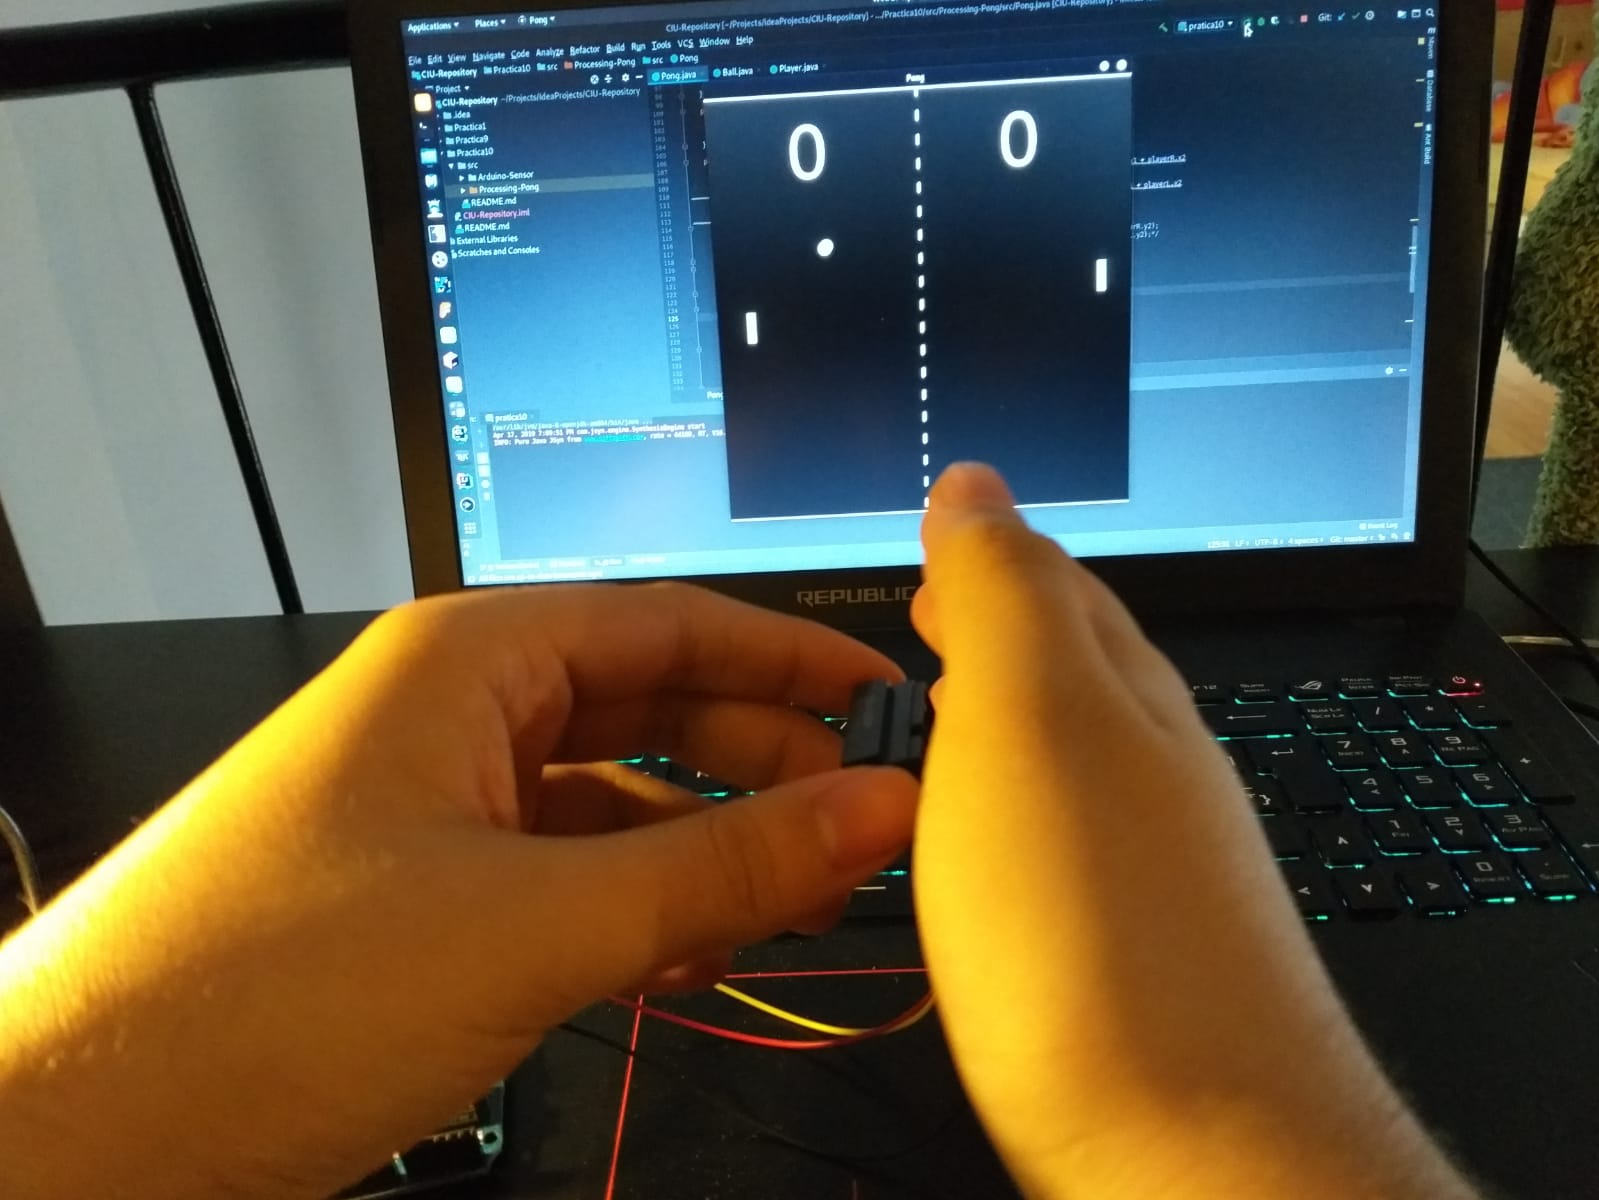
\includegraphics[width=0.75\textwidth]{project.jpeg}
		\caption{Integración de un sensor de proximidad con \textit{Processing}}
	\end{figure}
	\bibliography{Report10}
\end{document}